\documentclass[tikz]{standalone}
\usepackage{tikz}
\pagestyle{empty}

\tikzstyle{AR}+=[above right=1.5cm]
\tikzstyle{U}+=[anchor=south west]

\begin{document}
    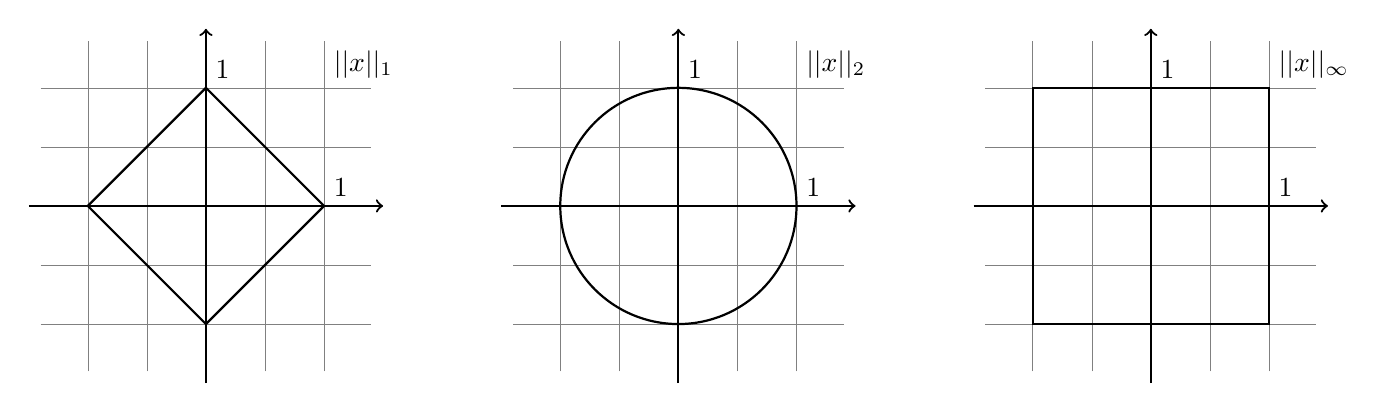
\begin{tikzpicture}[scale=1.5]
        \begin{scope}
            \draw[step=.5cm,gray,very thin] (-5.4,-1.4) grid (-2.6,1.4);
            \draw[thick,->] (-5.5,0) -- +(3,0) coordinate (x axis);
            \draw[thick,->] (-4,-1.5) -- +(0,3) coordinate (y axis);
            \draw[thick] (-5, 0) -- +(1,1) -- +(2,0) -- +(1,-1) -- cycle;
            \draw (-3,0) node[U]{$1$} (-4,1) node[U]{$1$} (-4,0) node[AR]{$||x||_1$};
        \end{scope}

        \begin{scope}
            \draw[step=.5cm,gray,very thin] (-1.4,-1.4) grid (1.4,1.4);
            \draw[thick,->] (-1.5,0) -- +(3,0) coordinate (x axis);
            \draw[thick,->] (0,-1.5) -- +(0,3) coordinate (y axis);
            \draw[thick] (0,0) circle (1cm);
            \draw (1,0) node[U]{$1$} (0,1) node[U]{$1$} (0,0) node[AR]{$||x||_2$};
        \end{scope}

        \begin{scope}
            \draw[step=.5cm,gray,very thin] (2.6,-1.4) grid (5.4,1.4);
            \draw[thick,->] (2.5,0) --  +(3,0) coordinate (x axis);
            \draw[thick,->] (4,-1.5) -- +(0,3) coordinate (y axis);
            \draw[thick] (3,-1) rectangle +(2,2);
            \draw (5,0) node[U]{$1$} (4,1) node[U]{$1$} (4,0) node[AR]{$||x||_\infty$};
        \end{scope}

    \end{tikzpicture}
\end{document}
